% ThaiEditBench --- ACL paper.  COMPILE WITH LuaLaTeX (not pdfLaTeX): Thai script
% needs fontspec + babel font-switching.  On Overleaf set the compiler to LuaLaTeX.
% Build:  lualatex -> biber/bibtex -> lualatex -> lualatex   (or latexmk -lualatex)
\documentclass[11pt]{article}

% "review" = anonymous + line numbers.  Switch to "final" / "preprint" later.
\usepackage[review]{acl}

\usepackage{microtype}
\usepackage{graphicx}
\usepackage{booktabs}
\usepackage{amssymb}
\usepackage{amsmath}

% Let a wide (two-column) table occupy more of a page top, so the leaderboard
% fits on the results page rather than spilling past the bibliography.
\renewcommand{\dbltopfraction}{0.92}
\renewcommand{\dblfloatpagefraction}{0.8}
\renewcommand{\topfraction}{0.9}
\renewcommand{\textfraction}{0.07}

% --- Fonts / scripts (LuaLaTeX or XeLaTeX only) -----------------------------
\usepackage[english]{babel}
\babelfont{rm}{TeX Gyre Termes}            % Times-like for Latin
% Auto-switch to a Thai font whenever Thai-script characters appear, so inline
% Thai needs no wrapping.  Requires a recent babel (Overleaf TeXLive is fine).
% The Thai font is BUNDLED in fonts/ (Noto Serif Thai), so this compiles anywhere
% without relying on a system/TeXLive copy of the font.
\babelprovide[import, onchar=ids fonts]{thai}
\babelfont[thai]{rm}[Path=fonts/, Extension=.ttf,
  UprightFont=NotoSerifThai-Regular, BoldFont=NotoSerifThai-Bold]{NotoSerifThai}
% ----------------------------------------------------------------------------

\title{ThaiEditBench: A Mechanism-Typed, Length-Stratified Benchmark\\
       for Thai Orthographic Error Correction}

\author{Anonymous ACL submission}

\begin{document}
\maketitle

\begin{abstract}
Thai is written without word boundaries and layers tone marks, silenced consonants, and
heavy loanword transliteration onto a Brahmic script. This produces orthographic error
mechanisms unlike those targeted by English grammatical error correction (GEC) or Chinese
spelling check (CSC). We present \textbf{ThaiEditBench}, a character-level Thai orthographic
error-correction benchmark with three components: (i) a principled \textbf{six-class
mechanism taxonomy} plus an etymology tag; (ii) \textbf{three length tiers} (sentence,
paragraph, and page) that isolate robustness to long, mostly-clean context; and (iii)
\textbf{contamination-robust construction}, in which errors are \emph{injected} into novel
clean text and \emph{mined} from Wikipedia cleanup-bot history, then screened by a
memorization probe. Because errors are introduced by construction, gold corrections are exact
and require no human annotation. Grading is at the character-cluster level with span-based
matching adapted from ERRANT.
Evaluating \textbf{16 models}, we find that (1) on this benchmark, correction is primarily a
\emph{detection} problem rather than a knowledge problem; (2) the evaluated Thai-specialized
models do not lead the strongest general models; and (3) long, mostly-correct context exposes
\textbf{over-edit accumulation} and clean-text fidelity failures that sentence-level evaluation
hides.
\end{abstract}

\section{Introduction}

Thai orthography is error-prone in script-specific ways: tone-mark selection and placement,
silenced-consonant marks, homophonous consonants, vowel-form confusions, consonant-cluster
metathesis, and inconsistent loanword transliteration. These are \textbf{character-level}
errors that turn on \textbf{specific mechanisms}, and Thai's lack of whitespace word
boundaries makes them hard to localize and score with token-based tools. Yet the resources to
study them are missing. Grammatical-error-correction benchmarks are English-centric
\citep{bryant-etal-2017-automatic,bryant-etal-2019-bea,napoles-etal-2017-jfleg}, and the
closest character-level analogue is Chinese spelling check
\citep{tseng-etal-2015-introduction,liu-etal-2011-visually}. For Thai, existing
error-annotated resources are social-media, informal, or learner-domain
\citep{lertpiya-etal-2020-thai,nakwijit-purver-2022-misspelling}, and there is no
formal-register, mechanism-typed, contamination-controlled orthographic benchmark.
Document-level and context-aware GEC study correction over long context
\citep{yuan-bryant-2021-document}, but no benchmark isolates length and error-sparsity
robustness for Thai orthographic correction.

\noindent\textbf{Contributions.}
(1)~\textbf{ThaiEditBench}, a character-level Thai orthographic correction benchmark: a
six-class mechanism taxonomy plus an etymology tag, \textbf{three length tiers} (sentence,
paragraph, page), built \textbf{contamination-robust by construction} (confusion-set injection
over novel clean text and Wikipedia cleanup-bot mining, memorization-probe screened) so gold is
exact and needs no human annotation.
(2)~An \textbf{ERRANT-style orthographic edit-typer for Thai} that aligns edits at TCC level
and labels each with one of the six mechanism classes, enabling \textbf{per-mechanism
span-F0.5} (cf.\ ChERRANT's dual-granularity scoring \citep{zhang-etal-2022-mucgec}). We use
it as a scoring and diagnosis instrument, not a general Thai grammatical error classifier.
(3)~A \textbf{16-model evaluation} yielding three findings: correction-is-detection, the
evaluated Thai-specialized systems do not lead, and over-edit accumulation under long context
in weaker models.
We release code, data, grader, edit-typer, and the variant map, anonymized for review:
\url{https://github.com/BlindReviewYN/ThaiEditingBench}.

\section{Related Work}

\noindent\textbf{GEC and CSC.} English grammatical error correction is evaluated with
span-based metrics. The M\textsuperscript{2} scorer matches a system's edits against gold edit
spans \citep{dahlmeier-ng-2012-better}, ERRANT (the ERRor ANnotation Toolkit) additionally
infers an error type for each edit automatically and reports an F0.5 score
\citep{bryant-etal-2017-automatic}, and GLEU measures
fluency \citep{napoles-etal-2015-ground}. ERRANT-style span matching aligns the wrong and
corrected text into a minimal set of edit spans, then credits a system for each gold span it
recovers with the correct replacement; we adapt this scheme to Thai TCC units
(Section~\ref{sec:typer}). Character-level Chinese spelling check is the closest task, scoring
position-based detection and correction F1 without word boundaries
\citep{tseng-etal-2015-introduction,wu-etal-2013-chinese,yu-etal-2014-overview}, with
confusion-set construction \citep{liu-etal-2011-visually} and the MuCGEC/ChERRANT
dual-granularity scorer \citep{zhang-etal-2022-mucgec}. ERRANT has been ported to Arabic
\citep{belkebir-habash-2021-automatic} and Korean \citep{yoon-etal-2023-towards}, but not Thai.
Wikipedia-revision mining of typo pairs is established for English
\citep{grundkiewicz-junczysdowmunt-2014-wiked} and Japanese
\citep{tanaka-etal-2020-building}.

\noindent\textbf{Thai NLP.} We build on PyThaiNLP for tokenization and dictionary tooling
\citep{phatthiyaphaibun-etal-2023-pythainlp} and on the Thai Character Cluster as the minimal
orthographic unit \citep{theeramunkong-etal-2000-character}. Prior Thai spelling correction
targets social text \citep{lertpiya-etal-2020-thai,lertpiya-etal-2023-progressively}, and
related work studies the semantics of Thai misspellings
\citep{nakwijit-purver-2022-misspelling}. The VISTEC-TP-TH-2021 Twitter corpus includes
misspelling detection and correction as well as word-segmentation annotation, but it is
informal Twitter text rather than a formal-register, mechanism-typed orthographic benchmark
\citep{limkonchotiwat-etal-2021-handling}.

\section{The ThaiEditBench Benchmark}

\subsection{Task}
Given a Thai passage containing character-level orthographic errors, return the passage with
those errors corrected and \textbf{nothing else changed}: no rewriting, re-spacing, numeral,
or punctuation edits. We score under a strict \textbf{minimal-edit contract}, where any change
to a non-erroneous span is an \emph{over-edit} and is penalized.

\subsection{Mechanism taxonomy}
We define six orthographic mechanism classes, each carrying an \textbf{etymology tag}: tone
mark, consonant-pair, silent-consonant, vowel, cluster or metathesis, and loanword
transliteration. Worked examples per class are in Appendix~\ref{app:taxonomy}. Canonical forms
are verified against the Royal Institute Dictionary (ORST). Class~6 is governed by a
\textbf{loanword-absorption rule}: only \emph{contemporary} foreign loans are class~6, while
long-integrated borrowings (Tamil, Khmer, Persian, and Sanskrit--Pali doublets) are treated as
native.

\subsection{Construction}
Two complementary sources both yield \textbf{construction-gold}. Applying the gold edits to an
item restores the clean original, which we verified holds for 100\% of items.
\begin{itemize}\itemsep2pt
\item \textbf{(a) Confusion-set injection.} A 1{,}044-pair $\times$ 6-class Thai confusion set
is injected into \emph{novel clean text} using \textbf{whole-token-run matching} (not
substring) to protect short valid forms. Each injected item records the Thai Character Cluster
(TCC) span, class, and etymology.
\item \textbf{(b) Cleanup-bot mining.} Real wrong$\to$correct pairs are mined from the edit
history of a Thai Wikipedia spelling-cleanup bot (RID-gated and misalignment-guarded),
following the revision-mining tradition
\citep{tanaka-etal-2020-building,grundkiewicz-junczysdowmunt-2014-wiked}.
\end{itemize}
\noindent\textbf{Registers.} The clean text spans news (thaisum), encyclopedic (Thai
Wikipedia), and government and legal (Royal Gazette, thaigov), all permissively
redistributable.

\subsection{Contamination control}
The benchmark reduces contamination risk by evaluating systems on \textbf{corrupted passages
that do not appear verbatim in the source corpora}. A residual risk remains: a model that
memorized a clean source passage could reconstruct it directly instead of detecting and
correcting the injected errors. We therefore run a \textbf{verbatim-continuation memorization
probe} on the source passages and hold the lowest-memorization material out from the public
release.

\subsection{Length tiers}
\label{sec:tiers}
The same pipeline produces three tiers that vary passage length and error sparsity.
\textbf{T1} (sentence) has 795 items of $\sim$100 characters each; \textbf{T2} (paragraph) has
223 items of $\sim$424 characters; and \textbf{T3} (page) has 124 items of $\sim$1{,}242
characters. Item counts are class-balanced across the six mechanisms, and full per-tier
statistics are in Appendix~\ref{app:construction}. The error budget is \textbf{dense at the
sentence level}, with roughly one error per 100 characters, and deliberately \textbf{sparse at
paragraph and page length}, where most sentences are clean distractors. T2 and T3 therefore
measure \textbf{precision under long correct context} (over-editing), not just recall, an axis
the CSC and GEC literature does not test.

\subsection{Quality control (fully automatic)}
\label{sec:qc}
Because errors are introduced by construction, the gold is exact. We add two automatic guards.
\begin{itemize}\itemsep2pt
\item \textbf{Cross-model consensus audit.} When at least $k{=}3$ of the 16 systems produce
the \emph{same} normalized output that differs from gold, we flag the item for review.
Consensus is a flagging heuristic, not proof of a gold defect. We drop the item only when the
agreed output is a residual \emph{source} typo that the construction-time filter missed. We
keep the other two cases: a \emph{shared miss}, where the consensus equals the corrupted input
and the gold is fine, and a \emph{systematic over-edit} on punctuation or register. The
classification is deterministic. The audit removed 24 of 819 (T1), 27 of 250 (T2), and 26 of
150 (T3) items, and post-audit no item is universally missed. The full protocol is in
Appendix~\ref{app:qc}.
\item \textbf{Variant reconciliation.} Spellings with two accepted forms are reconciled to the
gold form before scoring, token-aware and compound-safe. This covers orthographic doublets,
loanword transliterations, and an informal-to-formal pronoun pair, so a model is never penalized
for a legitimate variant.
\end{itemize}
Orthographic correction is essentially \textbf{single-reference}, since there is one correct
spelling, so we do not adopt multi-reference GEC machinery. Variant reconciliation covers the
few genuine alternatives.

\section{Evaluation Protocol}

\subsection{Metrics}
We grade at the TCC level \citep{theeramunkong-etal-2000-character} with ERRANT-style span
matching \citep{bryant-etal-2017-automatic}. The \textbf{primary metric is correction F1}:
minimal TCC edits are derived by aligning the wrong text against \emph{both} the gold and the
system output under the \textbf{same} Levenshtein alignment, so an output identical to the
reference scores exactly 1.0 (SIGHAN-CSC-comparable \citep{tseng-etal-2015-introduction}), and
we report it with a 95\% \textbf{item-bootstrap confidence interval}. \textbf{Detection F1}
credits the correct error site and ignores the replacement. \textbf{Clean-sentence fidelity}
is the fraction of error-free sentences left untouched, the exact and construction-grounded
precision signal for T2 and T3. We also report \textbf{per-mechanism span-F0.5} via the
edit-typer (Section~\ref{sec:typer}). Word-level GLEU is reported only as a supplementary metric in
Appendix~\ref{app:results}, because Thai word segmentation is unreliable for this task.

\subsection{ERRANT-style edit-typer}
\label{sec:typer}
We adapt the ERRANT/ChERRANT design
\citep{bryant-etal-2017-automatic,zhang-etal-2022-mucgec} to Thai orthography. For a (wrong,
correct) pair: extract edit spans at \textbf{TCC level} (the same alignment the grader uses),
expand each to its enclosing word (PyThaiNLP \texttt{newmm}
\citep{phatthiyaphaibun-etal-2023-pythainlp}), and label it with one of the six mechanism
classes (plus an edit-operation tag); class~6 is etymology-gated by a loan lexicon. This enables
\textbf{per-mechanism span-F0.5}. Its inventory is orthographic-mechanism-specific and reuses
the construction-time classifier, so we treat it as a \textbf{scoring instrument}, not a
general Thai grammatical error classifier.

\subsection{Models and inference}
We evaluate 16 models, each in a single fixed configuration, at temperature 0 where supported,
with one fixed Thai instruction prompt. The \textbf{frontier proprietary} models are GPT-5.5
(medium and high reasoning), Gemini~3.5~Flash, Claude Opus~4.7 (non-thinking), Claude
Sonnet~4.6 (non-thinking), and GPT-5.4-mini. The \textbf{open-weight} models are Gemma-4-31B,
DeepSeek~V4 Pro and Flash, GLM-5.1, MiniMax-M2.7, and Qwen3.6-35B-A3B. The \textbf{Thai-native}
models are Typhoon~2.5 (30B) and three ThaiLLM 8B-instruct models served through the national
ThaiLLM gateway, namely OpenThaiGPT, Typhoon-S, and THaLLE
\citep{pipatanakul-etal-2024-typhoon2,pipatanakul-etal-2026-typhoons}.

\section{Results and Analysis}

\subsection{Leaderboard}
The full leaderboard is Table~\ref{tab:leaderboard} (Appendix~\ref{app:results}), reporting
correction F1 across the three tiers (post-audit: $n = 795 / 223 / 124$). The frontier clusters at 0.95 to 0.97 on T1, and bootstrap CIs
separate three strata (frontier, then GLM, then the Thai-8B models and runaways). No single
model solves the entire T1 set, and no item is \emph{missed} by every model, so the gold is
clean post-audit yet retains per-model hard cases. \textbf{The benchmark discriminates}, and
the length-degradation slope (T1 to T3) is the sharpest discriminator (Section~\ref{sec:length}).

General frontier models dominate, while Thai-specialized models trail. Typhoon~2.5 scores
0.742 on T1 and 0.467 on T3, and the 8B national-gateway models score 0.74 to 0.78 on T1 but
fall to 0.45 to 0.62 on T3. The strongest \textbf{open-weight} model is a general 31B model,
Gemma-4. It is within CI of the frontier proprietary models on T1 and T2 and is the single
best model on the page tier (T3, 0.889). Under this setup the evaluated Thai-specialized systems
do not lead, and the gap widens with length. This comparison is confounded by differences in
model scale, serving stack, and inference configuration, so it is not evidence about
Thai-specialized pretraining in general.

\subsection{Correction is a \emph{detection} problem}
Decompose every gold edit (T1) into \textbf{fixed}, \textbf{wrong\_corr} (right site, wrong
fix), and \textbf{missed} (Table~\ref{tab:decomp}). Across \textbf{all 16 models},
\texttt{wrong\_corr} never exceeds 0.036, while \texttt{missed} carries essentially the entire
error budget. Once a model \emph{notices} an error it almost always fixes it correctly. What
separates models is \textbf{error discrimination}, not knowledge of correct spellings. This
reframes the implicit assumption in correction-centric CSC work.

\begin{table}[t]
\centering\small
\begin{tabular}{@{}lrrr@{}}
\toprule
model & fixed & wrong\_corr & missed \\
\midrule
GPT-5.5 (high)   & 0.993 & 0.000 & 0.007 \\
Gemma-4-31B      & 0.956 & 0.004 & 0.040 \\
Qwen3.6-35B-A3B  & 0.817 & 0.018 & 0.165 \\
Typhoon 2.5 30B  & 0.764 & 0.036 & 0.201 \\
\bottomrule
\end{tabular}
\caption{Gold-edit outcome decomposition (T1). \texttt{wrong\_corr} stays near zero for every
model; the budget is \texttt{missed}.}
\label{tab:decomp}
\end{table}

\subsection{Length robustness}
\label{sec:length}
Sentence-tier rank does \textbf{not} predict paragraph or page behaviour, and the
\textbf{degradation slope from T1 to T3 is the sharpest discriminator}
(Figure~\ref{fig:degradation}a). The frontier loses only 0.10 to 0.12 correction F1
(GPT-5.5-med $0.969{\to}0.856$; Gemma-4 $0.950{\to}0.889$), while weak models fall off a cliff
(Typhoon~2.5 $0.742{\to}0.467$; Qwen $0.705{\to}\mathbf{0.308}$, a drop of 0.40). The long
tiers also expose over-editing. We measure it as the over-edit rate per 10{,}000 clean TCCs,
which factors out how much clean text a model is exposed to. This rate is roughly flat or falls
across tiers (Qwen $105{\to}107{\to}65$; Typhoon~2.5 $57{\to}33{\to}27$;
Figure~\ref{fig:degradation}b), so over-editing accumulates with length through exposure rather
than through a rising false-positive rate. The discriminating signal is the \emph{level} of that
rate, not its slope: weak models over-edit at 5 to 20 times the frontier's per-unit rate, which
stays below $\sim$15 per 10{,}000 clean TCCs at every tier. Clean-sentence
\textbf{fidelity} tells the same story. The frontier holds at or above 0.95 throughout, while
weak models sit at 0.78 to 0.90 regardless of length. \textbf{Over-editing and missing are two
faces of the same weak discrimination}: a model that cannot tell correct from incorrect both
misses real errors and rewrites correct text. The exception is instructive. \textbf{Gemini 3.5
Flash keeps high recall at T3, fixing 0.985 of gold edits, yet drops to 0.819 correction F1
purely on precision}. It is the one frontier model whose page-tier score is limited by
over-editing rather than by detection.

\subsection{Per-mechanism difficulty}
Class~6 (loanword) is the hardest mechanism, with $\sim$0.81 of edits fixed versus $\sim$0.86
to 0.90 for tone marks, consonant pairs, and silent-consonant marks. The failure is again
\textbf{missed}, not miscorrected: models are least certain that a transliteration is wrong.
But the \emph{ranking} within class~6 does \textbf{not} favour Thai-native models. Difficulty
is a property of the \textbf{mechanism}, not of cross-lingual knowledge. Register agrees:
loanword-dense encyclopedic text is hardest (recall $\sim$0.71 to 0.82) versus government and
news text ($\sim$0.83 to 0.90).

\section{Conclusion}
ThaiEditBench is a mechanism-typed, length-stratified, contamination-robust benchmark for Thai
orthographic correction, released with an ERRANT-style edit-typer for per-mechanism scoring.
Across 16 models it reframes correction as a \textbf{detection} problem, shows that the
evaluated \textbf{Thai-specialized systems do not lead}, and surfaces \textbf{over-edit
accumulation} under long context in weaker models.

\section*{Limitations}
\textbf{Sparse error density (primary).} The long tiers (T2 and T3) are deliberately sparse,
with 1 to 3 errors scattered across otherwise-clean passages, to isolate precision under long
correct context. We therefore do \textbf{not} test \textbf{high error-density} regimes such as
heavy-typo input, degraded OCR, or L2 writing, where errors co-occur, interact, mask one
another, and correction order matters. Extending ThaiEditBench to dense multi-error passages,
and testing whether the detection-not-knowledge result survives when errors crowd each other,
is the most important next step.

\textbf{Reasoning-mode not swept.} Models run in mixed default configurations, so the
leaderboard compares default behaviour rather than a controlled thinking-on or thinking-off
contrast.

\textbf{Configured-system comparison.} Each system is evaluated under one fixed configuration.
Reasoning modes, token budgets, provider defaults, serving stacks, and model scale are not
controlled, so the leaderboard reflects configured-system behaviour rather than an intrinsic
ranking of base-model capability.

\textbf{Length-normalized over-editing.} Raw over-edits per item rise with passage length,
because longer passages expose more clean text where a false positive can occur. We therefore
report the over-edit rate per clean TCC alongside the absolute per-passage count, and we base
rate claims on the normalized metric while reading the absolute count as user-visible
accumulation.

\textbf{Minimal-edit vs fluency boundary.} Occasionally a frontier ``over-edit'' is actually
catching a residual error that our injection-gold did not mark, which slightly understates the
best models.

\textbf{No human inter-annotator agreement.} Gold is construction-based, either injected or
mined, and audited automatically. We run no human annotation pass, so no inter-annotator
agreement is reported. This is sound for \emph{injected} errors, where the gold is exact by
construction, but the mechanism-class labels and the mined items rest on automatic typing
rather than on measured human consensus.

\bibliographystyle{acl_natbib}
\bibliography{custom}

\appendix

\section{Mechanism taxonomy in detail}
\label{app:taxonomy}
Each class is defined by the orthographic \emph{mechanism} of the fault, not its surface
character. Multiple worked examples per class:
\begin{itemize}\itemsep1pt
\item \textbf{1 tone mark:} ค๊ะ$\to$คะ, น๊ะ$\to$นะ, จั๊กจั่น$\to$จักจั่น, กระทั้ง$\to$กระทั่ง
\item \textbf{2 consonant-pair:} กฏหมาย$\to$กฎหมาย, กบฎ$\to$กบฏ, อากาส$\to$อากาศ
\item \textbf{3 silent-consonant:} กลยุทธ$\to$กลยุทธ์, ขาดดุลย์$\to$ขาดดุล, เท่ห์$\to$เท่
\item \textbf{4 vowel:} สังเกตุ$\to$สังเกต, มาตราฐาน$\to$มาตรฐาน, ฉะเพาะ$\to$เฉพาะ
\item \textbf{5 cluster/metathesis:} กระทันหัน$\to$กะทันหัน, กระบังลม$\to$กะบังลม
\item \textbf{6 loanword:} กราฟฟิค$\to$กราฟิก, กงศุล$\to$กงสุล, ลิ๊งค์$\to$ลิงก์
\end{itemize}
\textbf{Loanword-absorption rule.} Only \emph{contemporary} foreign loans, chiefly modern
English technical and commercial terms (กราฟิก, ดิจิทัล, ลิงก์), are class~6. Long-integrated
borrowings are treated as \textbf{native} even though etymologically foreign: Portuguese
(กะละแม), Burmese (กะปิ), Mon (กะพง), Khmer (กบฏ), and Tamil, Persian, and Sanskrit--Pali
doublets. Borderline cases (e.g.\ กงสุล, \emph{consul}) are resolved by ORST listing $+$
Wiktionary borrowed-term categories, and the tag is recorded per item so the rule is auditable.

\section{Gold quality control and the consensus audit}
\label{app:qc}
\textbf{Why construction-gold still needs a cleanup pass.} Injection guarantees that applying
the gold edits recovers the clean original (verified 100\%), so the \emph{injected} error's
correction is exact. It does \textbf{not} guarantee that the \textbf{source passage was
typo-free}: the permissive corpora contain a small rate of residual orthographic errors. When
an item's source carries such a residual typo, the gold inherits it, so a model that fixes
\emph{that} genuinely wrong span is unfairly scored as a miss or an over-edit. We remove these
automatically.

\textbf{Cross-model consensus audit.} For every item we pool all 16 outputs
(variant-reconciled) and look for a \emph{consensus} output, the same normalized string from
at least $k{=}3$ systems, that differs from gold. The discrimination is three-way.
(i)~If the consensus equals the corrupted input, this is a \emph{shared miss}, the gold is
correct, and we \textbf{keep} the item.
(ii)~If the consensus is a punctuation, whitespace, or register variant, this is a systematic
\emph{over-edit}, the precision signal we want, and we \textbf{keep} it.
(iii)~If the consensus is a \emph{different} spelling fix at an unmarked span, this is a
residual \emph{source} typo, and we \textbf{drop} it. Only case (iii) is a gold defect, and
the explicit test of whether the consensus equals the input prevents conflating it with shared
misses and over-pruning. The audit removed 24 (T1), 27 (T2), and 26 (T3) items, for example
ทั้งสิน$\to$ทั้งสิ้น, ปฏิเศษ$\to$ปฏิเสธ, and โดบ$\to$โดย, all residual \emph{source} typos.
\textbf{Post-audit invariant:} no item in any tier is missed by all 16 models. This is the
signature that residual gold defects are gone while genuinely hard items remain. The drop list
is committed by the deterministic three-way rule above. The audit also ships with a
self-contained HTML review view (colored gold-vs-consensus diffs, with \textsc{drop},
\textsc{keep}, and \textsc{variant} badges) for optional inspection and reproducibility.

\section{Construction details}
\label{app:construction}
Confusion set: 1{,}044 canonical pairs $\times$ 6 classes, RID-verified against
\texttt{thai\_orst\_words} (87.5\%; misses are modern loanwords absent from the offline ORST),
each tagged with etymology and edit-operation. Injection uses \textbf{whole-token-run matching}
so the 51 valid short forms ($\le 3$ characters) that coincide with a confusion target are
never corrupted. Cleanup-bot mining draws pairs from the \texttt{usercontribs} history of a
single Thai Wikipedia spelling-cleanup bot, RID-gated and misalignment-guarded; these are held
out from the public release. A verbatim-continuation \textbf{memorization probe} (Typhoon~2.5
30B) scores all sources LOW (mean longest-common-prefix 0.003 to 0.017), and the
lowest-memorization text is held out from the public release.

\begin{table}[t]
\centering\small\setlength{\tabcolsep}{4pt}
\begin{tabular}{@{}llrrrc@{}}
\toprule
tier & unit & items & chars & err/it & news/gov/enc \\
\midrule
T1 sent.  & 1 sent.          & 795 & 100     & 1.23 & 275/368/152 \\
T2 para.  & $\approx$5 sent.  & 223 & 424     & 1.24 & 80/79/64 \\
T3 page   & $\approx$15 sent. & 124 & 1{,}242 & 1.56 & 42/43/39 \\
\bottomrule
\end{tabular}
\caption{Per-tier statistics (post-audit; Section~\ref{sec:qc}). Counts are class-balanced across the
six mechanisms (T1: 115 to 211 edits per class). The described tiers are 100\% confusion-set
injection; cleanup-bot material is held out from the public release.}
\label{tab:tiers}
\end{table}

\paragraph{Release and license.} We release the benchmark for research use under CC BY-SA (data)
and the MIT license (code), consistent with the permissive redistribution terms of the source
corpora; the anonymized review release is linked in the contributions (Section~1).

\section{Full results}
\label{app:results}
\begin{table*}[t]
\centering\small
\begin{tabular}{@{}lcccccc@{}}
\toprule
model & T1 det & T1 corr & T2 corr & T2 fid & T3 corr & T3 fid \\
\midrule
GPT-5.5 (high)        & \textbf{0.973} & \textbf{0.973} & \textbf{0.969} & \textbf{0.990} & 0.855 & 0.974 \\
GPT-5.5 (med)         & 0.969 & 0.969 & 0.955 & 0.983 & 0.856 & 0.971 \\
Claude Opus 4.7       & 0.971 & 0.968 & 0.948 & 0.986 & 0.848 & 0.974 \\
Gemini 3.5 Flash      & 0.969 & 0.965 & 0.960 & 0.983 & 0.819 & 0.960 \\
Gemma-4-31B           & 0.954 & 0.950 & 0.954 & 0.988 & \textbf{0.889} & 0.981 \\
GPT-5.4-mini          & 0.959 & 0.949 & 0.917 & 0.986 & 0.853 & \textbf{0.988} \\
Claude Sonnet 4.6     & 0.952 & 0.947 & 0.906 & 0.977 & 0.824 & 0.972 \\
DeepSeek V4 Flash     & 0.952 & 0.947 & 0.945 & 0.986 & 0.828 & 0.966 \\
DeepSeek V4 Pro       & 0.928 & 0.926 & 0.926 & 0.970 & 0.746 & 0.954 \\
GLM-5.1               & 0.851 & 0.846 & 0.812 & 0.961 & 0.665 & 0.954 \\
Typhoon-S 8B$^\dagger$         & 0.788 & 0.782 & 0.702 & 0.961 & 0.619 & 0.965 \\
THaLLE 8B$^\dagger$            & 0.758 & 0.749 & 0.595 & 0.775 & 0.517 & 0.829 \\
Typhoon 2.5 30B$^\dagger$      & 0.776 & 0.742 & 0.631 & 0.881 & 0.467 & 0.896 \\
OpenThaiGPT v7.2$^\dagger$     & 0.755 & 0.741 & 0.477 & 0.887 & 0.454 & 0.896 \\
MiniMax-M2.7          & 0.747 & 0.740 & 0.720 & 0.974 & 0.470 & 0.968 \\
Qwen3.6-35B-A3B       & 0.721 & 0.705 & 0.383 & 0.776 & 0.308 & 0.836 \\
\bottomrule
\end{tabular}
\caption{Leaderboard: correction and detection F1 and clean-sentence fidelity across the three
length tiers. \textbf{Bold} $=$ column best; $\dagger$ $=$ Thai-native. Per-model CIs, detection
F1, ChERRANT span-F0.5, and per-class recall are released with the data. The frontier T1 CI width
is $\sim\pm0.01$. \textbf{Gemma-4-31B leads T3} (0.889), clear of the GPT-5.5 pair near
0.855, so a \emph{general} open-weight model is the most robust at length.}
\label{tab:leaderboard}
\end{table*}
\begin{figure*}[t]
\centering
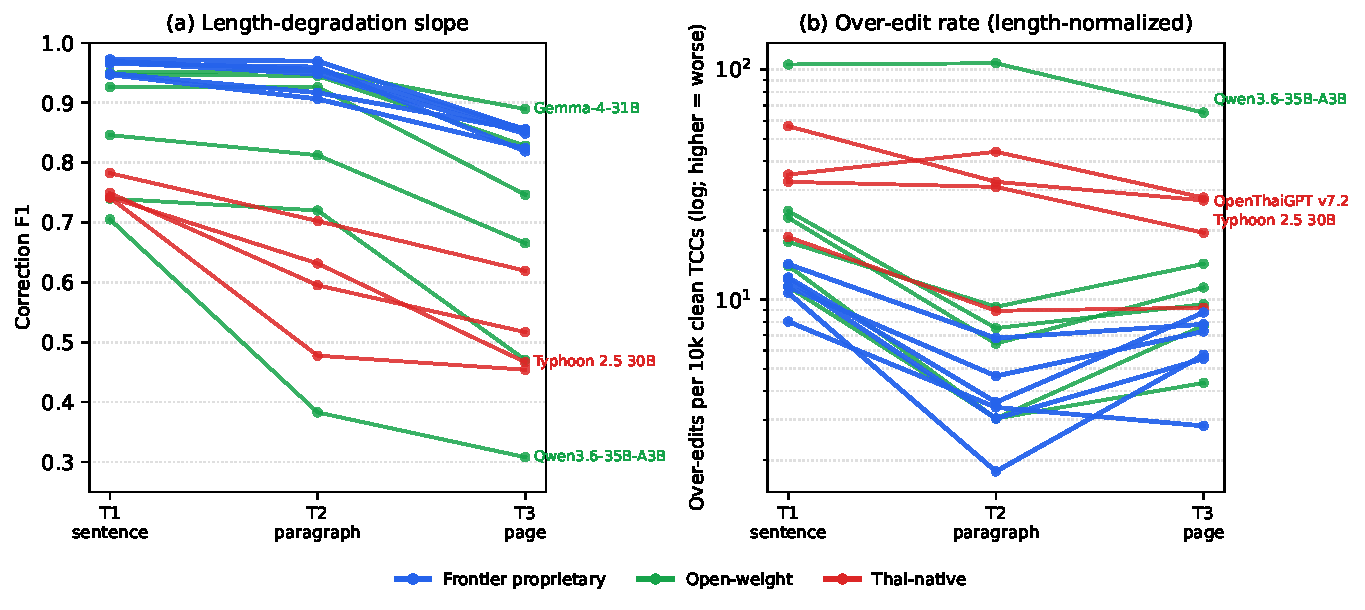
\includegraphics[width=\textwidth]{fig1-degradation.pdf}
\caption{Length robustness. \emph{(a)}~Correction-F1 slope from T1 to T3. The frontier (blue)
and the strongest open-weight model (Gemma-4, green) stay high while weak models slope off.
\emph{(b)}~Over-edit rate per 10{,}000 clean TCCs on a log scale, where higher is worse. The
rate is roughly flat across length, so the per-passage accumulation (the absolute counts below)
reflects text exposure rather than a rising false-positive rate. Weak models over-edit at many
times the frontier's per-unit rate at every tier.}
\label{fig:degradation}
\end{figure*}

\textbf{Pooled per-class outcome split (T1, all 16 models).}
\begin{center}\small\setlength{\tabcolsep}{3pt}
\begin{tabular}{@{}lrrrr@{}}
\toprule
class & gold edits & fixed & wrong\_corr & missed \\
\midrule
1 tone     & 2{,}608 & 0.896 & 0.011 & 0.092 \\
2 consonant& 2{,}192 & 0.876 & 0.006 & 0.117 \\
3 silent-consonant & 2{,}640 & 0.887 & 0.010 & 0.103 \\
4 vowel    & 2{,}896 & 0.857 & 0.002 & 0.140 \\
5 cluster  & 3{,}392 & 0.863 & 0.012 & 0.126 \\
6 loanword & 1{,}968 & 0.808 & 0.003 & 0.189 \\
\bottomrule
\end{tabular}
\end{center}
\textbf{Over-edits per 100 items across tiers (absolute accumulation).}
\begin{center}\small
\begin{tabular}{@{}lrrr@{}}
\toprule
model & T1 & T2 & T3 \\
\midrule
GPT-5.5 (med)    & 7  & 8   & 41  \\
Gemma-4-31B      & 6  & 8   & 32  \\
GLM-5.1          & 10 & 23  & 106 \\
Typhoon 2.5 30B  & 32 & 82  & 201 \\
OpenThaiGPT v7.2 & 20 & 110 & 206 \\
Qwen3.6-35B-A3B  & 59 & 268 & 484 \\
\bottomrule
\end{tabular}
\end{center}
\textbf{Over-edit rate per 10{,}000 clean TCCs (length-normalized; the
Figure~\ref{fig:degradation}b data).} The per-unit rate is roughly flat or falls across tiers,
so the per-item growth above reflects text exposure, not a rising false-positive rate.
\begin{center}\small
\begin{tabular}{@{}lrrr@{}}
\toprule
model & T1 & T2 & T3 \\
\midrule
GPT-5.5 (med)    & 12.3  & 3.0   & 5.5  \\
Gemma-4-31B      & 11.4  & 3.0   & 4.3  \\
GLM-5.1          & 17.8  & 9.3   & 14.3 \\
Typhoon 2.5 30B  & 56.8  & 32.6  & 27.0 \\
OpenThaiGPT v7.2 & 35.0  & 44.0  & 27.8 \\
Qwen3.6-35B-A3B  & 105.4 & 106.8 & 65.1 \\
\bottomrule
\end{tabular}
\end{center}
\textbf{Register effect (pooled correction recall, T1/T2/T3).} encyclopedic 0.82/0.79/0.71;
news 0.87/0.85/0.76; government 0.89/0.90/0.83. Per-model $\times$ class correction recall and
ChERRANT span-F0.5 per type are released with the data. \textbf{Word-level GLEU} is released as
a supplementary comparability metric only. We exclude it from the main metrics because Thai
word segmentation is unreliable for this task.

\section{Prompt and inference}
\label{app:prompt}
A single fixed Thai instruction prompt is used for all models. It asks the model to return the
passage with orthographic errors corrected and \textbf{nothing else changed}, explicitly
forbidding spacing, punctuation, and numeral edits. Temperature is 0 where supported. Claude
models use the Anthropic Message Batches API in non-thinking mode. GPT-5.x models use the
Responses API at the stated reasoning effort with a 3k-token budget. Open reasoning models run
in native thinking mode with large token budgets, and token-runout counts as a failure.
ThaiLLM-gateway models are reached with a browser User-Agent header, because the gateway WAF
otherwise blocks the default SDK agent.

\end{document}
